\section{Análisis de diagramas de dispersión}
\subsection{Lectura temporal con IMERG}
IMERG muestra dos máximos estacionales: abril--mayo (medias de 273,27 y 257,47~mm/mes) y octubre--noviembre (276,25 y 276,03~mm/mes). Los meses medios más secos son enero (144,68), julio (153,95) y agosto (154,74~mm/mes). Este patrón describe el ciclo observado por el producto y no demuestra una causa climática por sí solo.

El máximo mensual de IMERG es noviembre de 2008 (431,15~mm/mes), pero Q no está disponible ese mes; se conserva la lluvia y no se inventa caudal. El mínimo es diciembre de 2015 (56,10~mm/mes; Q=29,70~m$^3$/s). Con P25=152,59 y P75=262,82~mm/mes, el episodio seco más persistente es mayo--septiembre de 2015 (cinco meses, media 98,86~mm/mes), mientras el húmedo más persistente es febrero--junio de 2022 (cinco meses, media 293,36~mm/mes).

Los años con mayor precipitación media IMERG son 2008, 2011 y 2022, y 2015 es el más seco; son contrastes aparentes entre años, no una tendencia demostrada. En los 285 meses simultáneos, la correlación IMERG--Q es 0,63; con IMERG retrasado un mes es 0,61 y con dos meses 0,32. La asociación parece concentrarse en el mismo mes o en una escala menor que un mes, pero no identifica causalidad ni separa el efecto de almacenamiento, regulación y ciclo anual compartido.

\subsection{Agregación mensual, escorrentía y temperatura}
Para meses completos, con $P_d$ como precipitación diaria en mm, $Q_d$ como caudal medio diario en m$^3$/s y $n_m$ como número de días del mes, se usan
\[
P_m=\sum_{d\in m}P_d,\qquad \overline{Q}_m=\frac{1}{n_m}\sum_{d\in m}Q_d.
\]
Para comparar precipitación y escorrentía en láminas equivalentes, el caudal diario se convierte con el área de drenaje $A=2797,19$~km$^2$:
\[
R_m=\frac{86,4}{A}\sum_{d\in m}Q_d\quad [\mathrm{{mm/mes}}].
\]
La serie R del informe ya se calculó con esa expresión; por tanto no es una observación independiente de Q. No se debe repetir la conversión por área si el caudal ya estuviera expresado como lámina diaria.

La fuente original disponible contiene Tmin y Tmax diarios de MSWX, pero no una temperatura media directamente observada. Se grafica de manera provisional $T_{\mathrm{media,est}}=(T_{\min}+T_{\max})/2$, identificada como estimada. No se presenta como ERA5-Land/ERA5 ni como observación directa; debe contrastarse o reemplazarse con una fuente de temperatura media directa antes de una interpretación climática final.

\begin{figure}[H]\centering
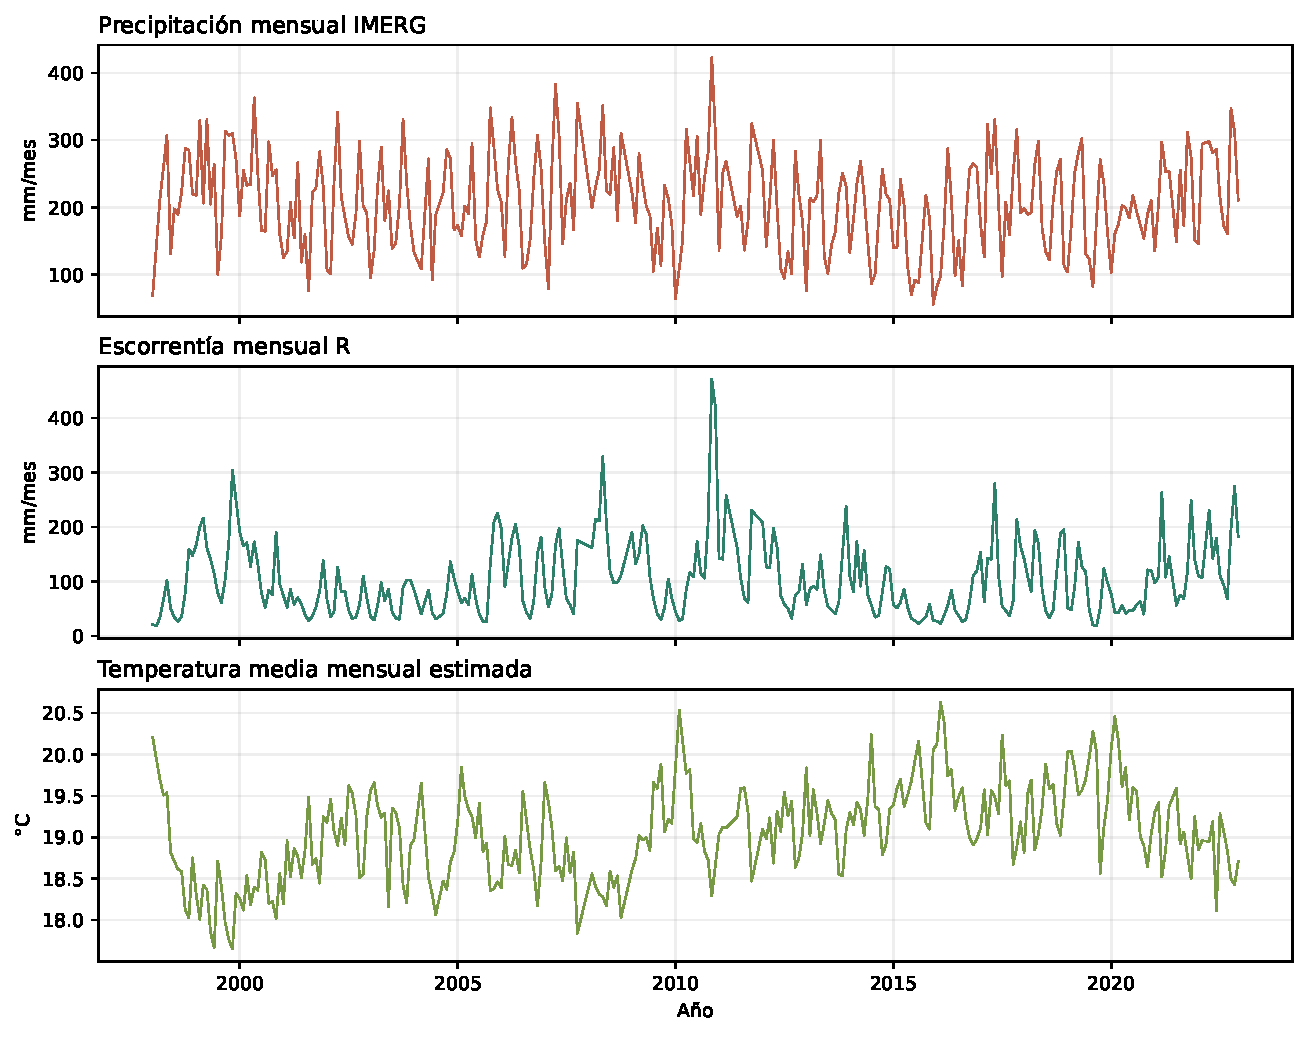
\includegraphics[width=\linewidth]{figuras/imerg_r_temperatura_comun.pdf}
\caption{IMERG, escorrentía mensual R y temperatura media mensual estimada, para los 285 meses completos simultáneos. IMERG y R están en mm/mes.}
\end{figure}

\subsection{IMERG: distribución y control descriptivo}

En este apartado se presentan únicamente serie, distribución, caja y estadísticos de IMERG; no se superponen con CHIRPS. El catálogo identifica 172 instalaciones dentro o en el borde de la cuenca, de las cuales 131 están clasificadas como lluvia. Ese conteo solo indica cobertura potencial: no demuestra continuidad de las series ni que esas estaciones hayan sido usadas como datos de entrada.

\begin{figure}[H]\centering
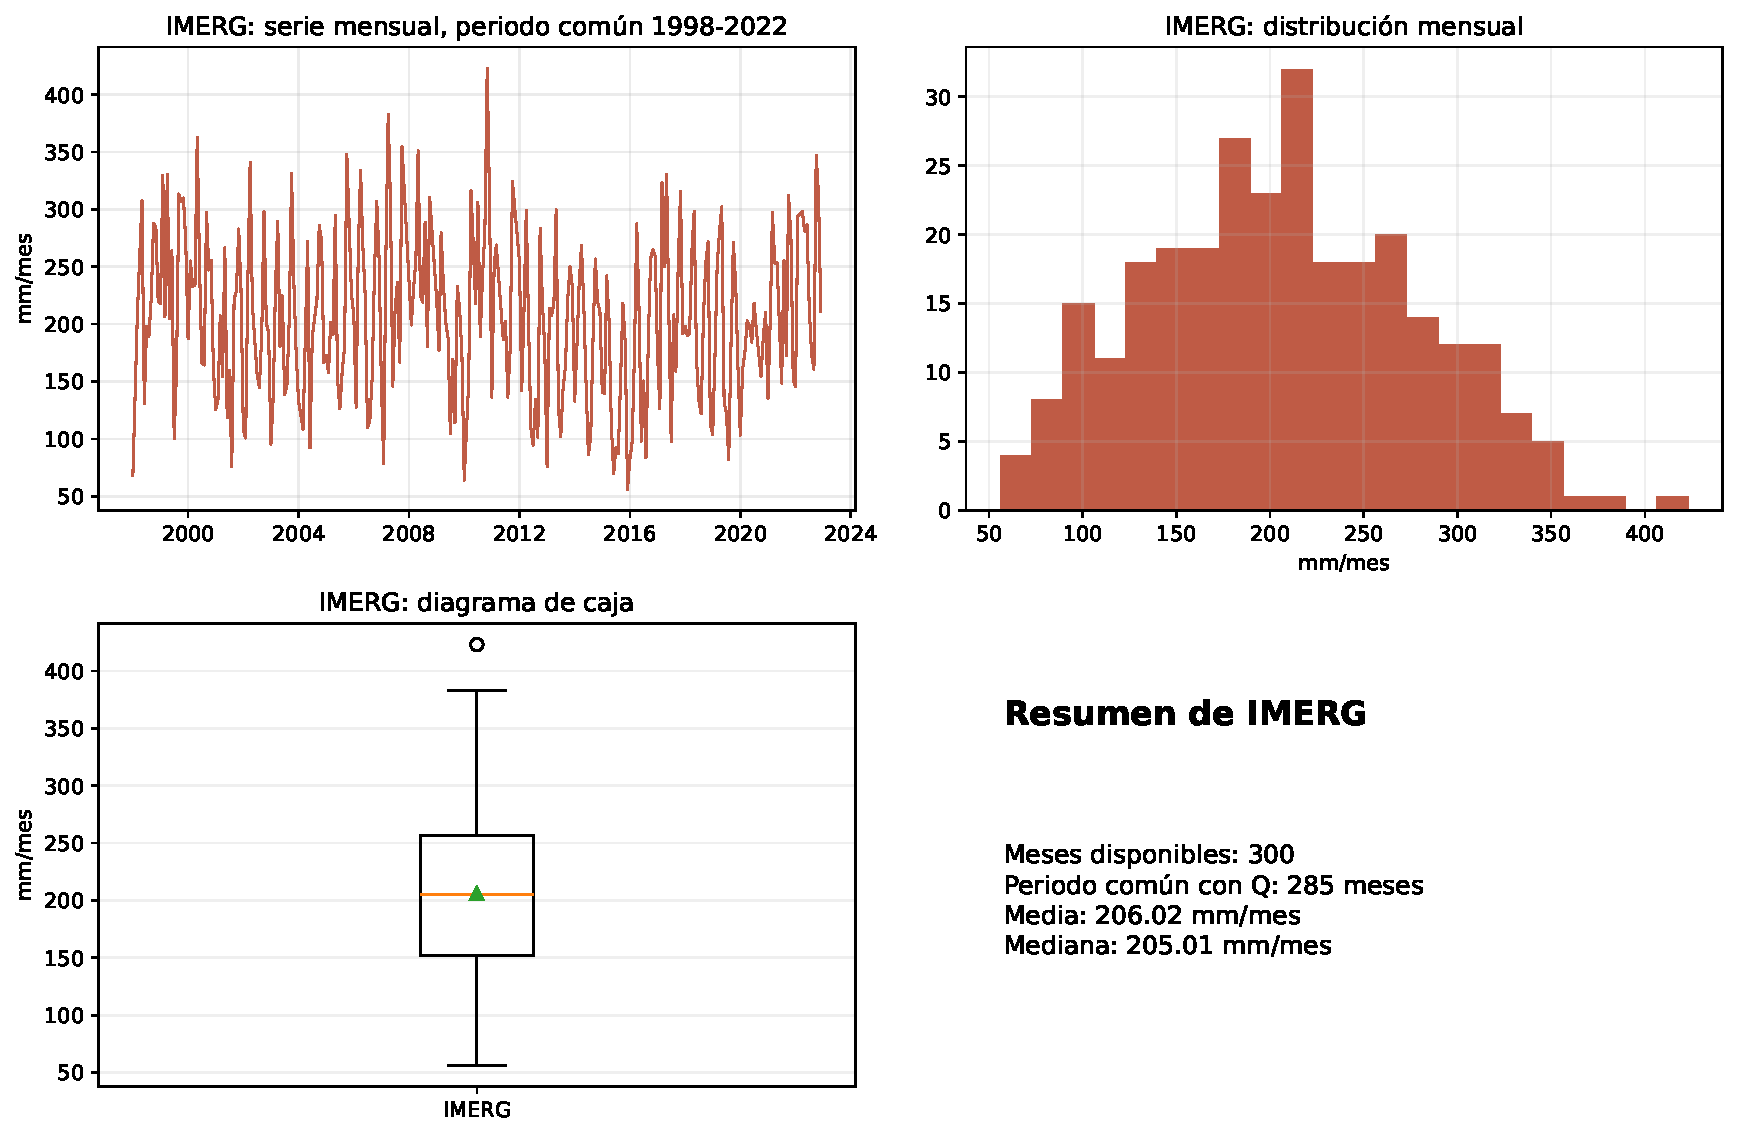
\includegraphics[width=\linewidth]{figuras/imerg_complemento.pdf}
\caption{IMERG incorporado al análisis: serie cronológica, distribución, diagrama de caja y resumen del periodo común.}
\end{figure}

\subsection{Diagramas requeridos con IMERG y lluvia local}
Se construyeron los tres diagramas solicitados: IMERG frente a lluvia local, lluvia local frente a caudal Q e IMERG frente a caudal Q. Los puntos se colorean por mes calendario. La estación Zaragoza-AUT ofrece solo 22 meses simultáneos completos en esta descarga; por eso las dos relaciones que incluyen lluvia local son exploratorias y no representan toda la serie 1998--2022.

\begin{figure}[H]\centering
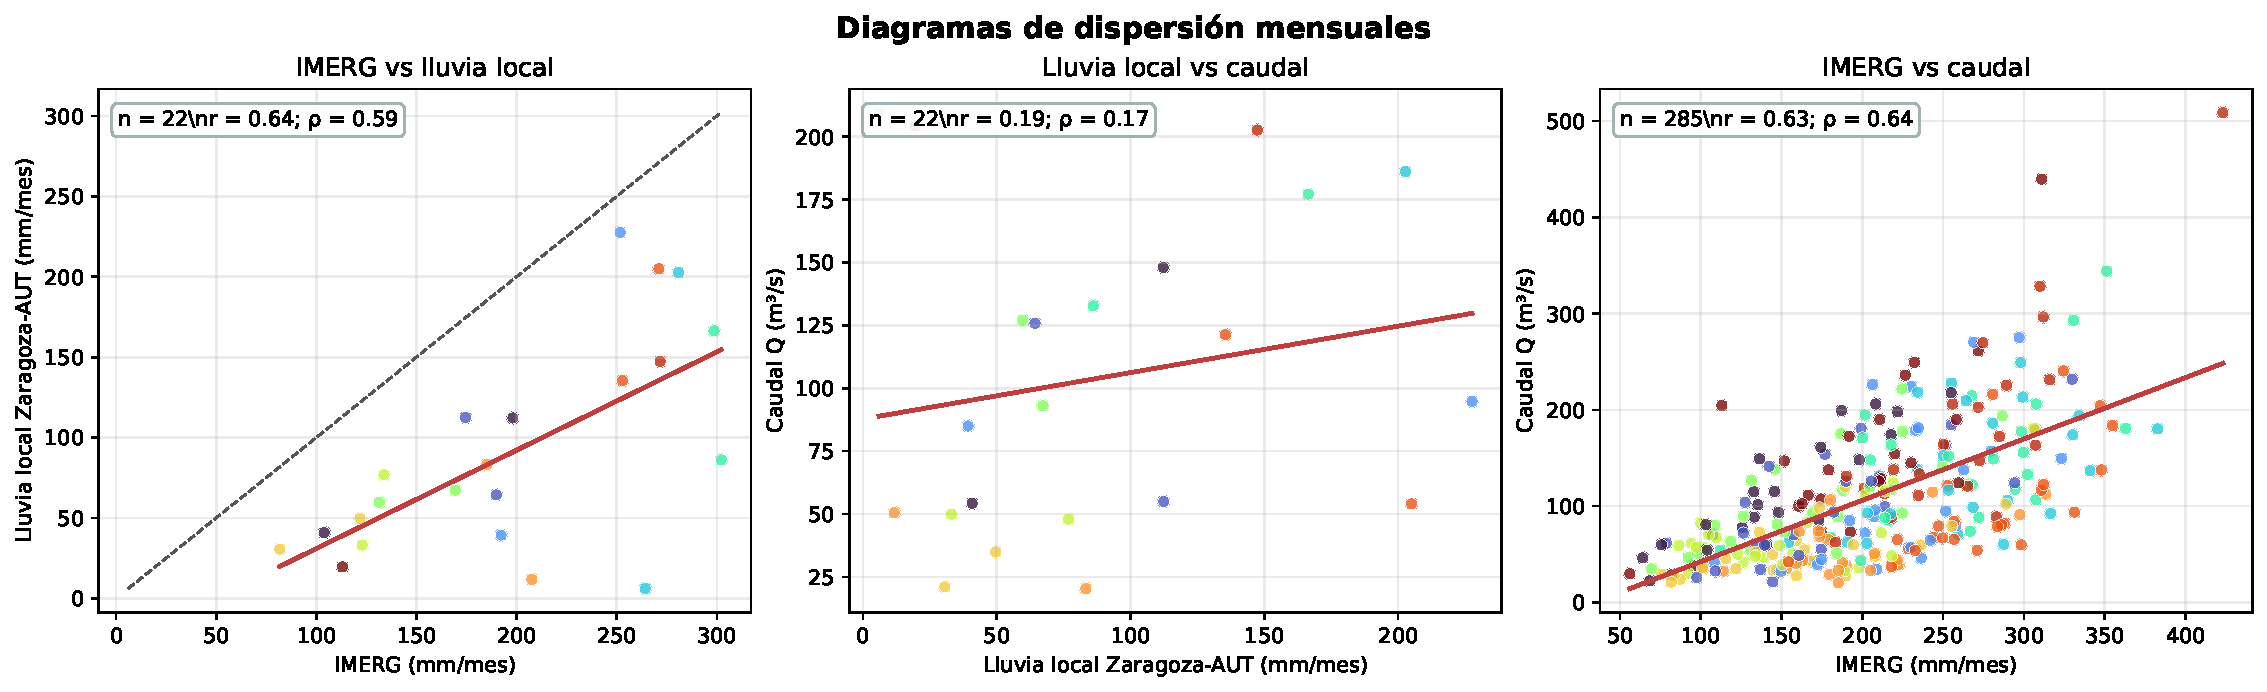
\includegraphics[width=\linewidth]{figuras/dispersiones_requeridas.pdf}
\caption{Diagramas de dispersión requeridos. La línea discontinua en IMERG--lluvia local es 1:1.}
\end{figure}

Para IMERG--lluvia local, Pearson es 0,64 y Spearman 0,59; el sesgo IMERG menos local es +106,42 mm/mes, MAE 106,42 mm/mes y RMSE 120,17 mm/mes. Lluvia local--Q tiene Pearson 0,19 y Spearman 0,17 (n=22); IMERG--Q tiene Pearson 0,63 y Spearman 0,64 (n=285). Son estadísticas descriptivas; falta comparar anomalías mensuales y evaluar rezagos sin usar precipitación futura.

\subsection{CHIRPS--Q: análisis paralelo}
Se conservan P CHIRPS acumulada y Q observado de 485 meses completos,
entre enero de 1981 y diciembre de 2022. CHIRPS es una estimación espacial, no
una estación terrestre. Se interpreta en paralelo con IMERG: ninguna de las dos fuentes
sustituye a la otra. Los pares IMERG--lluvia local, IMERG--Q y lluvia local--Q
se presentan arriba; para IMERG aún faltan las comparaciones con anomalías mensuales
y el análisis de rezagos.

\begin{figure}[H]\centering
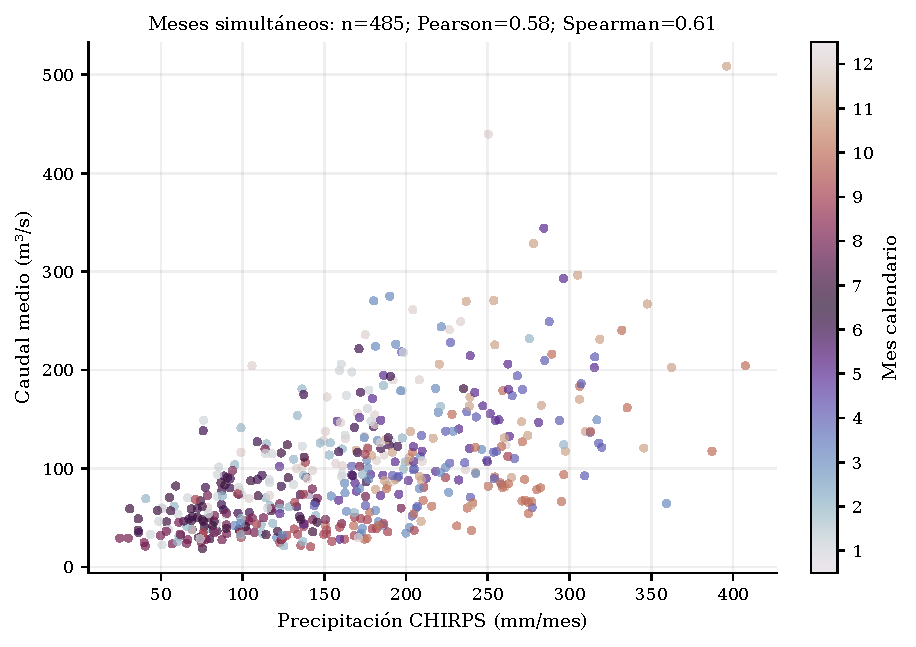
\includegraphics[width=.85\linewidth]{figuras/dispersion_CHIRPS_caudal.pdf}
\caption{Dispersión de P CHIRPS y Q observado. El color identifica el mes calendario.}
\end{figure}

Con valores mensuales Pearson es 0,58 y Spearman es 0,61. Parte de la asociación puede provenir del ciclo anual común. Al quitar el promedio histórico de cada mes calendario, Pearson es 0,56 y Spearman es 0,58. Las anomalías responden mejor a si un mes más lluvioso de lo habitual coincide con caudal mayor de lo habitual.

\begin{center}\small\begin{tabular}{rrrr}\hline
Rezago P (meses) & Meses emparejados & Pearson & Spearman \\ \hline
0 & 485 & 0,58 & 0,61 \\
1 & 484 & 0,61 & 0,68 \\
2 & 483 & 0,27 & 0,33 \\
3 & 482 & -0,06 & -0,07 \\
\hline\end{tabular}\end{center}
El mayor Pearson a escala mensual se observa con P rezagada 1 mes(es) (0,61). Esto no demuestra un tiempo físico de respuesta: los promedios mensuales pueden ocultar respuestas de días/semanas y Q depende además de humedad antecedente, almacenamiento y operación.

No se reportan p-valores simples porque los meses consecutivos son dependientes. Estas correlaciones no prueban causalidad ni son un modelo de pronóstico; se requieren rezagos diarios, validación temporal y otras variables.
